\section{Transition-Level Transfer}
Transition-level \simtoreal deals with dynamics modeling: how the state evolves under actions. The simulator’s physics (mass, friction, contacts) rarely match reality precisely, especially in contact-rich or deformable tasks. This is often the hardest gap to bridge, since even small physics errors can accumulate.

A common strategy is \emph{dynamics randomization}: sampling simulation parameters (mass, inertia, friction coefficients, gravity, etc.) from a broad distribution during training. This approach generates a policy robust to a variety of dynamics. It was famously used by OpenAI in their bipedal robot and Dactyl hand experiments, randomizing parameters like joint friction, motor strength, and even gravity to ensure the policy did not rely on any precise setting\cite{Akkaya2019}. Tan et al. similarly randomized terrain friction and actuator gains for quadruped locomotion, leading to successful transfer of galloping and trotting gaits\cite{Tan2018}. Figure~\ref{fig:quadruped} shows an example: a Minitaur robot learned to gallop in simulation and executed the gait in reality. While not a plot, this juxtaposition of sim vs real performance (from Tan et al.) illustrates that well-randomized training can produce controllers that behave similarly in both domains.

\begin{figure}[H]
    \centering
    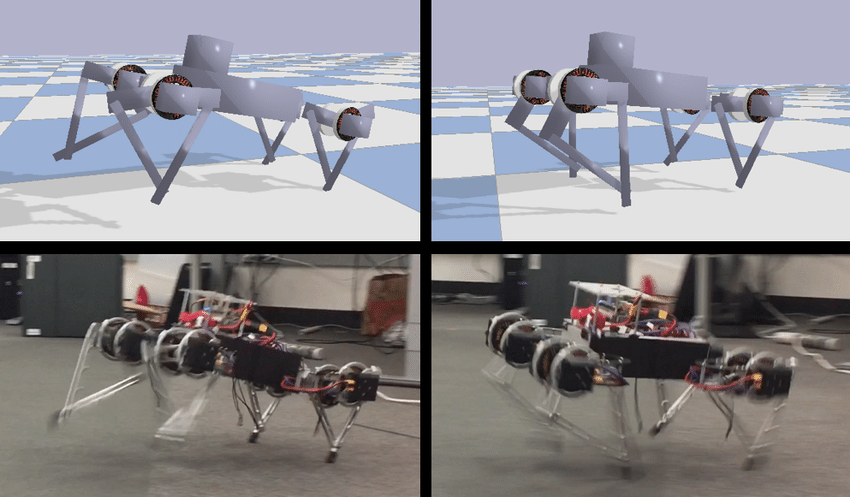
\includegraphics[width=0.95\linewidth]{figures/figMinitaurGallop.png}
    \caption{Quadruped locomotion learned in simulation and deployed on hardware.  (Top) Simulated Minitaur robot in galloping gait (four frames at different times). (Bottom) The real Minitaur performing a learned gallop. (\emph{Source:} Tan et al.~\cite{Tan2018}.)}
    \label{fig:quadruped}
\end{figure}

However, randomization has limits: if the real-world dynamics lie outside the randomized range, or if the gap is \emph{irreducible} (e.g.\ complex contact physics that simulators cannot represent), performance suffers. Moreover, randomization offers little guidance for refining sim parameters post-transfer. An alternative is \emph{system identification (SysID)}: using real-world data to calibrate the simulator. Early SysID efforts involved manual tuning of physical parameters. Recent approaches, such as SimOpt~\cite{Chebotar2019}, automate this loop: a policy is trained in sim, tested on hardware, and the parameter distribution is updated to reduce trajectory mismatch. Grounded Simulation Learning~\cite{Hanna2017} further refines transitions by inserting learned corrections directly into the simulation dynamics.

More recently, \emph{task-driven adaptation} frameworks aim to optimize simulation not for physical realism but for real-world task performance. AdaptSim~\cite{Ren2023} exemplifies this approach. It alternates between training a policy in simulation, testing on hardware, and adjusting the simulation distribution via a learned adaptation policy. The result is a task-driven refinement of simulation. Figure~\ref{fig:adapt_sim} (adapted from Ren et al.) illustrates this in a real scooping task, where each iteration significantly improves success rate.

\begin{figure}[H]
    \centering
    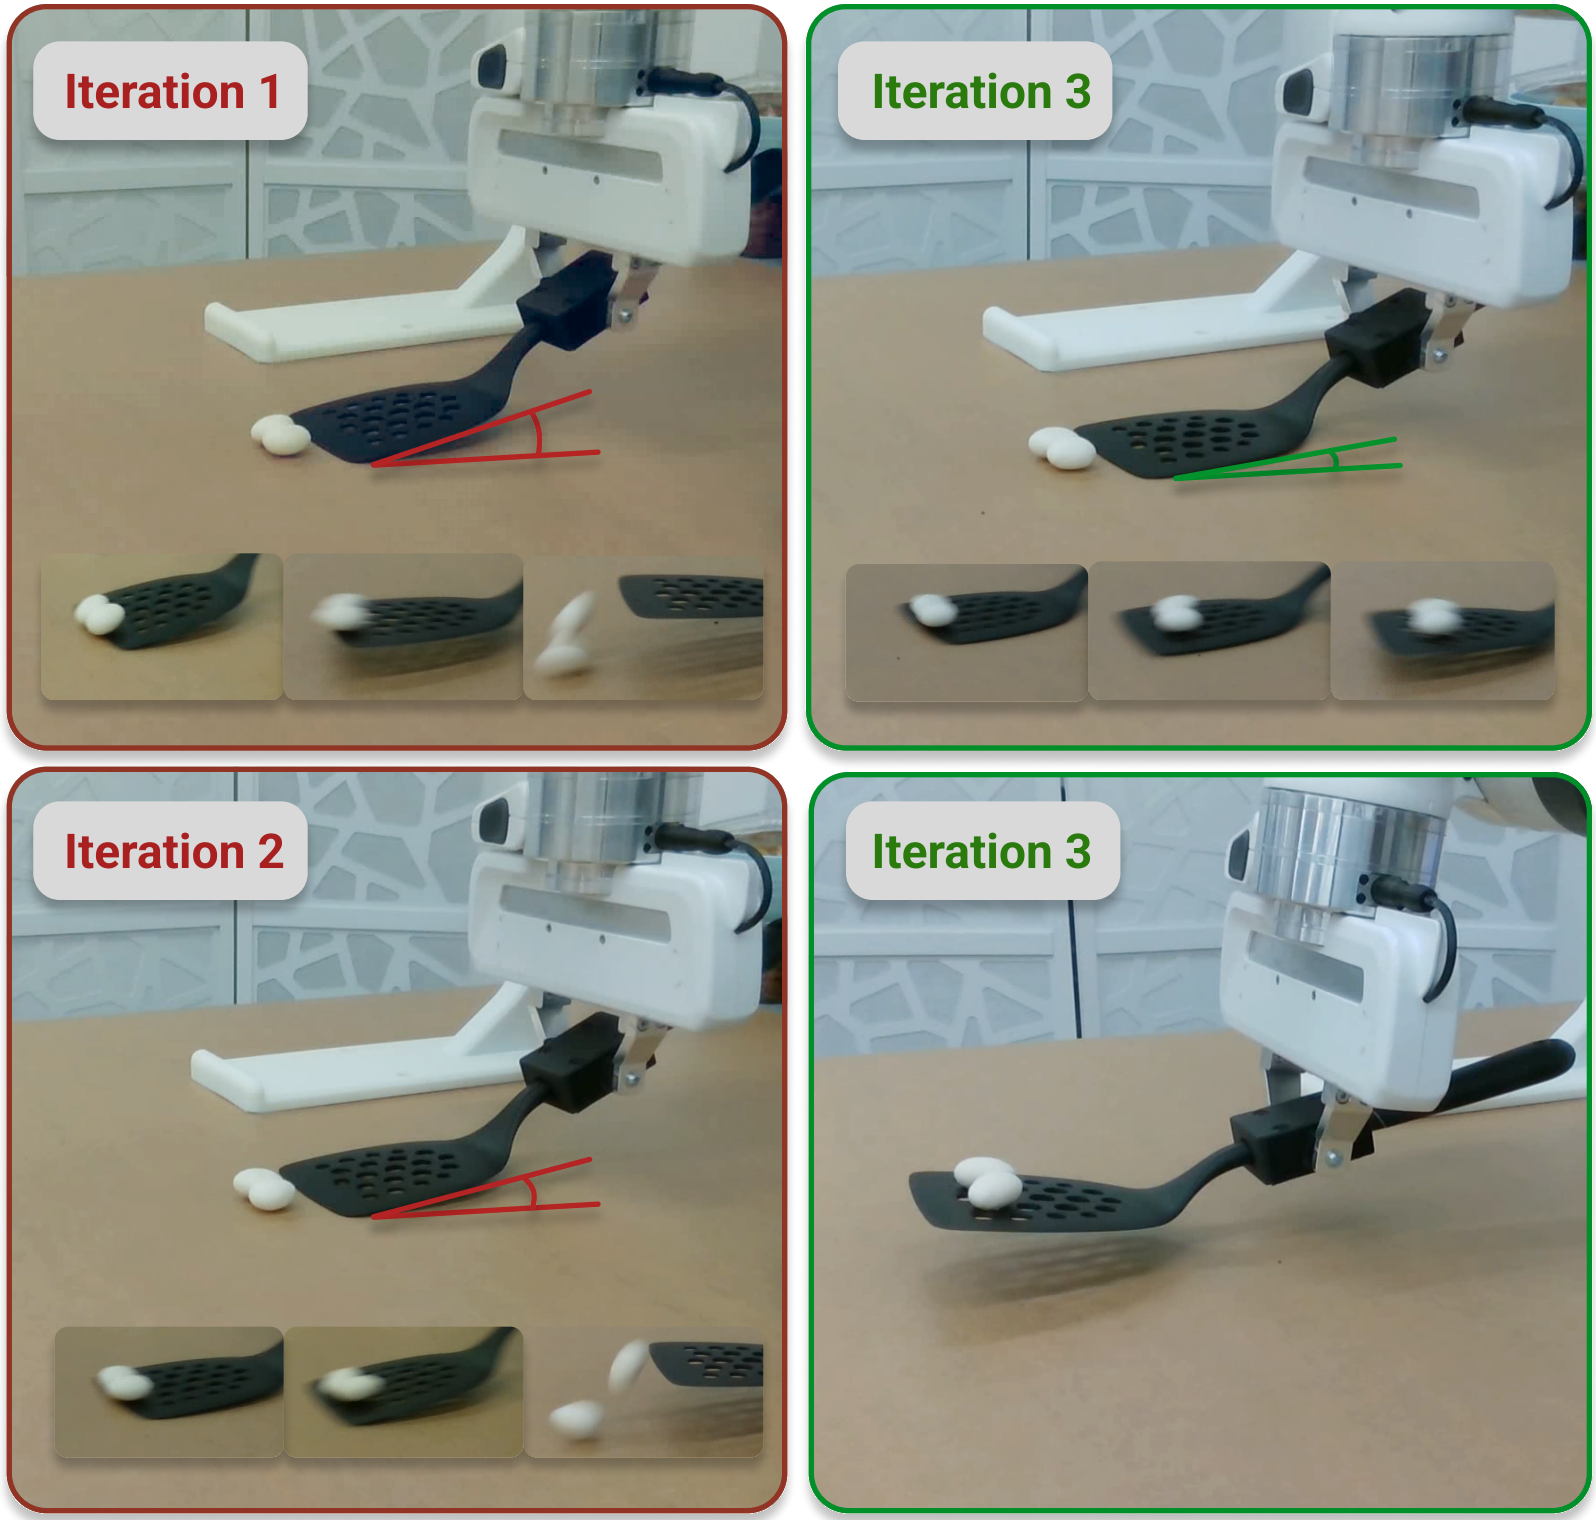
\includegraphics[width=0.95\linewidth]{figures/figAdaptSim.png}
    \caption{Adaptive simulation improvement on a real scooping task (Ren et al.~\cite{Ren2023}). The robot attempts to scoop marshmallows with a spatula under varying simulation parameters. Iteration~1 (red) shows poor performance; by Iteration~3 (green) the learned policy successfully scoops the object consistently. (Credit: Adapted from Ren et al.~\cite{Ren2023}.)}
    \label{fig:adapt_sim}
\end{figure}

In summary, transition-level transfer methods range from broad dynamics randomization to data-driven calibration. Randomization is simple and scalable but may fail in unmodeled regions. SysID improves accuracy but depends on stable measurements and repeated hardware access. Task-driven methods like AdaptSim optimize directly for task outcomes, offering an efficient balance. Across studies, hybrid pipelines—randomization followed by adaptation—consistently outperform isolated strategies\cite{Chebotar2019,Ren2023}.

\paragraph{Evaluation.} Dynamics randomization has proven effective in locomotion and manipulation tasks (e.g., OpenAI Dactyl~\cite{Akkaya2019}, Minitaur robot~\cite{Tan2018}). However, it assumes that the true real-world parameters are covered by the randomized distribution, which is not always guaranteed. System identification methods such as SimOpt~\cite{Chebotar2019} provide more accurate sim-real alignment by directly minimizing discrepancy through real-world trials. While this improves transfer performance, it requires repeated access to hardware and assumes stable and measurable dynamics.
